We tackle the same problem as is found in \cite{Zhang_2015_CVPR, guan2021understanding} of
subitization. However, there are a few differences between this implementation and each of those
implementations. In contrast to \cite{Zhang_2015_CVPR}, they work with a much wider definition of
subitization, in which the counter can count every kind of object; the domain is not restricted to
objects of the same type or roughly of the same type. We use a dataset that is extremely trivial
(uniform shapes in an image with a black backgroud) relative to their dataset. Though ambiguous
according to \cite{subitizingdefinition}, we believe that theirs is the correct interpretation,
especially from personal experience. Therefore, their problem is more difficult in this respect.
However, they stick with the common mindset of four objects being the maximum subitization
capability, and so compare their results to that limit (again, with a single category that pertains
to images with four or more objects). We do not believe this is a thorough test of the capabilities
of neural networks, and (though this fact was not a motivation for us) we take a stab at the neural
network learning to count an arbitrary number of objects. However, ``arbitrary'' does not mean
boundless as there can only be so many shapes within an image (a strong upper bound would be the
number of pixels in the image, but that is not a supremum). Both \cite{Zhang_2015_CVPR} and our work
attempt to detect objects using a classifier trained to count. However, our method performs the
localization as a byproduct of the second derivative of counting, which, although not exactly clear
due to time limits we had and ambiguity in the paper, differs from their methods; one of them uses
the output of the model as a guide for a separate counting method, for example.

With respect to \cite{guan2021understanding}, they make much stronger claims that this author feels
comfortable with. We aim to show that these networks can indeed subitize (up to a
object-dissimilarity limit), regardless of whether or not it is terribly accurate. Further, they
pose this problem as determining connected components, which allows them to make a claim that one
connecting pixel should be considered as merging two components into one. We think this is a dubious
argument, mostly because that for the example that they show~\cite{guan2021understanding}[figure
12], the vast majority of people would not likely be able to see the pixel-wide connection, and
therefore four separate components would have been the guess by most. Coincidentally, we also happen
to look at shapes, although we try to mix in different kinds and sizes of shapes into the same
image; they do try different sizes, but the sampling process is different (which we will use in our
implementation as a potential solution to poor saliency output).






The definition of our problem is as follows: given an image and a network, can we train the network
to successfully count shapes in a subitization fashion? The shapes were automatically generated with
random positioning; shape overlap detection was performed with the recommended\cite{viaforshapely}
Shapely\cite{shapely} package, and any overlap rejected that shape's location. Two possible shapes,
triangles and squares\footnote{This may be Professor David Crandall's idea} can be generated. Images
were drawn and saved with Pillow~\cite{imagesinpython}. Larger shapes resulted in proper learning;
we had no luck with smaller shapes. The network is a convolutional network, with no other layers
besides activation functions and a linear layer at the end to output a single
ReLU\cite{pmlr-v15-glorot11a}\footnote{This reference is commonly pointed to as the source of
ReLU}-filtered number. This is done because the network~\cite{szegedy2014going} they use in
\cite{10.1007/978-3-319-46487-9_48} does as well (except for the output layer). The loss function is
mean squared error, with the ground truth being the raw number of each kind of shape (this is in
contrast to \cite{Zhang_2015_CVPR}, which had separate classes that represented different counts).
Because the images are automatically generated, we are able to use extremely large datasets, which
may not be a reasonable expectation when training on non-artificial data. For now, we stick with
shapes as it is a simplified problem for which a proof-of-concept could lead to further research
into whether the concept can be applied in the real world (not just from a subitization standpoint,
but also from a detection one as well). We used Chainer~\cite{tokui2019chainer} to implement our
research in this section, as well as CuPy~\cite{cupy_learningsys2017}, NumPy~\cite{2020NumPy-Array},
and Python 3~\cite{language}. There was previous code that addressed this topic based on
PyTorch~\cite{NEURIPS2019_9015}; we did use it to some extent, but it was rewritten to use Chainer
later on. This code may have used Nesterov momentum instead.

\subsection{Detecting Shapes}
\label{detectingshapes}

To perform the detection step, a trained network\footnote{trained with small batch sizes as we found
this useful for some reason; it could be that small batch sizes increase variance, which results in
kind of a simulated annealing-like behavior} and an image are used to generate a saliency map via
the method described in \cite{simonyan2014deep}. However, instead of backpropagating from the
correct class's output (there is no concept of ``class'' in our network), we backpropagate from the
addition of all the outputs (which ideally would give us the total number of shapes), one output
squares and one for triangles. This addition occurs (most likely; thank the author's short memory)
because the aim is to detect \textit{all} shapes within the image, not just one type; however, it
would be good to see if saliency for a single shape type could be used (depending on the success of
the original method, of course).

The detection step comes in by exploiting the (yet unproven) property that the gradient of one pixel
depends on the value of another. Ideally, if the derivative of the saliency of the pixel w.r.t.
another pixel changes, then that implies that the changing value of the latter pixel (for this
example, it decreases to become more like the background) causes the former to take on more of a
representational burden in order to keep the object count up. However, it is possible that every
pixel in the image can change the second derivative of the target pixel. To see why, let's look at
the first derivative w.r.t. the image ($f$ is the sum over the estimated shape count, $x_i$ is
subpixel $i$ of image $x$, and $a_k$ is the output of layer $k$ for image $x$):
\[
    \frac{\partial f}{\partial x_i} = \frac{\partial f}{\partial a_k} \frac{\partial a_k}{\partial x_i}
\]
If we take the partial derivative of $\frac{\partial f}{\partial x_i}$ w.r.t. subpixel $j$, we see
that the product rule gives us non-zero values for some or all parts of the domain following what is
shown in section \ref{gradientmagnitudereduction}; the difference here is that we don't use a
non-linear loss function, so at least one activation function for this network \textit{must} be
non-linear (even if the function is piecewise, as described in \ref{gradientmagnitudereduction}) for
this to be true. We do not go over why not all layers have to have a non-zero second derivative in
that section (although work on the topic of \ref{gradientmagnitudereduction} likely preceded, and
therefore was the foundation of, this the idea of the type of activation causing second-order
issues), so we will do that here. Here is the analytical derivation of the second derivative:
\begin{multline*}
    \frac{\partial}{\partial x_j}     \frac{\partial a_4}{\partial a_3} \frac{\partial a_3}{\partial a_2} \frac{\partial a_2}{\partial a_1} \frac{\partial a_1}{\partial x_i} = \\[10pt]
    \frac{\partial f_3}{\partial x_i}  \left( \frac{\partial}{\partial x_j} \frac{\partial a_4}{\partial a_3} \right)       +       \frac{\partial a_4}{\partial a_3} \left( \frac{\partial}{\partial x_j} \frac{\partial f_3}{\partial x_i} \right)\\[10pt] 
    = \frac{\partial f_3}{\partial x_i}  \left( \frac{\partial}{\partial x_j} \frac{\partial a_4}{\partial a_3} \right)       +       \frac{\partial a_4}{\partial a_3}         \left[     
                \frac{\partial f_2}{\partial x_i}  \left( \frac{\partial}{\partial x_j} \frac{\partial a_3}{\partial a_2} \right)       +       \frac{\partial a_3}{\partial a_2} \left( \frac{\partial}{\partial x_j} \frac{\partial f_2}{\partial x_i} \right)
      \right]\\[10pt]
    = \frac{\partial f_3}{\partial x_i}  \left( \frac{\partial}{\partial x_j} \frac{\partial a_4}{\partial a_3} \right)       +       \frac{\partial a_4}{\partial a_3}         \left[     
                \frac{\partial f_2}{\partial x_i}  \left( \frac{\partial}{\partial x_j} \frac{\partial a_3}{\partial a_2} \right)       +       \frac{\partial a_3}{\partial a_2}          \left[
                        \frac{\partial f_1}{\partial x_i}  \left( \frac{\partial}{\partial x_j} \frac{\partial a_2}{\partial a_1} \right)       +       \frac{\partial a_2}{\partial a_1} \left( \frac{\partial}{\partial x_j} \frac{\partial f_1}{\partial x_i} \right)
                \right]
      \right]\\[10pt]
    = \frac{\partial f_3}{\partial x_i}  \left( \frac{\partial}{\partial x_j} \frac{\partial a_4}{\partial a_3} \right)       +       \frac{\partial a_4}{\partial a_3}         \left[     
                \frac{\partial f_2}{\partial x_i}  \left( \frac{\partial}{\partial x_j} \frac{\partial a_3}{\partial a_2} \right)       +       \frac{\partial a_3}{\partial a_2}          \left[
                        \frac{\partial f_1}{\partial x_i}  \left( \frac{\partial}{\partial x_j} \frac{\partial a_2}{\partial a_1} \right)       +       \frac{\partial a_2}{\partial a_1} \left( \frac{\partial}{\partial x_j} \frac{\partial a_1}{\partial x_i} \right)
                \right] 
      \right]
\end{multline*}
We can simplify this rather complex series of additions, and this looks like
\begin{multline*}
     \frac{\partial f_3}{\partial x_i}  \left( \frac{\partial}{\partial x_j} \frac{\partial a_4}{\partial a_3} \right)       +       \frac{\partial a_4}{\partial a_3}         \left[     
                \frac{\partial f_2}{\partial x_i}  \left( \frac{\partial}{\partial x_j} \frac{\partial a_3}{\partial a_2} \right)       +       \frac{\partial a_3}{\partial a_2}          \left[
                        \frac{\partial f_1}{\partial x_i}  \left( \frac{\partial}{\partial x_j} \frac{\partial a_2}{\partial a_1} \right)       +       \frac{\partial a_2}{\partial a_1} \left( \frac{\partial}{\partial x_j} \frac{\partial a_1}{\partial x_i} \right)
                \right] 
      \right]\\[10pt]
     = \frac{\partial f_3}{\partial x_i}  \left( \frac{\partial}{\partial x_j} \frac{\partial a_4}{\partial a_3} \right)       +       \frac{\partial a_4}{\partial a_3}         \left[     
                \frac{\partial f_2}{\partial x_i}  \left( \frac{\partial}{\partial x_j} \frac{\partial a_3}{\partial a_2} \right)       +
                         \frac{\partial a_3}{\partial a_2} \frac{\partial f_1}{\partial x_i}  \left( \frac{\partial}{\partial x_j} \frac{\partial a_2}{\partial a_1} \right)       +        \frac{\partial a_3}{\partial a_2} \frac{\partial a_2}{\partial a_1} \left( \frac{\partial}{\partial x_j} \frac{\partial a_1}{\partial x_i} \right)
       \right]\\[10pt]
     = \frac{\partial f_3}{\partial x_i}  \left( \frac{\partial}{\partial x_j} \frac{\partial a_4}{\partial a_3} \right)       +    
                \frac{\partial a_4}{\partial a_3} \frac{\partial f_2}{\partial x_i}  \left( \frac{\partial}{\partial x_j} \frac{\partial a_3}{\partial a_2} \right)       +
                         \frac{\partial a_4}{\partial a_3} \frac{\partial a_3}{\partial a_2} \frac{\partial f_1}{\partial x_i}  \left( \frac{\partial}{\partial x_j} \frac{\partial a_2}{\partial a_1} \right)       +
                                \frac{\partial a_4}{\partial a_3} \frac{\partial a_3}{\partial a_2} \frac{\partial a_2}{\partial a_1} \left( \frac{\partial}{\partial x_j} \frac{\partial a_1}{\partial x_i} \right)
\end{multline*}
We can expand this process to any number of layers. However, if each activation function has a
second derivative of $0$, the whole equation collapses to $0$; we discuss why this is relevant and a
problem shortly. If the last activation function's gradient has a gradient that is non-zero, then we
cannot guarantee the network's complete second derivative will end up being zero at some subpixel
$x_j$. This is essentially the same point that \ref{gradientmagnitudereduction} makes (and it may
have been based on it too). This conclusion requires that the derivatives of the derivatives of an
activation with respect to another evaluate (for example, $\left( \frac{\partial}{\partial x_j}
\frac{\partial a_4}{\partial a_3} \right)$) to zero. This happens to be the case because the second
derivative between two layers is zero, and the left-over derivative of the incoming set of
activations w.r.t. $x_j$ due to the chain rule application are nullified because it is multiplied by
the aforementioned second derivative. So, avoiding zero-valued second derivatives is necessary (one
non-zero second derivative will possibly result in a non-zero, end-to-end second derivative because
every addition in the above equation could give us something non-zero)\footnote{Stefan Lee confirmed
my math (at least for ReLU) as he also believed that $\frac{\partial^2 f}{\partial x_i}$ is required
to be non-zero}.

\subsection{Algorithm}
\label{algorithm}

Now that we have established the basic concepts and requirements for our localization procedure, we
can outline ways in which detection may happen. A way that we attempted (but were never able to
fully iron-out) and inspired by the thresholding used in \cite{reeves}[3:58] is that we take the
highest saliency~\cite{simonyan2014deep} value (which corresponds to a certain pixel $i$), and then
calculate the second derivative of that value w.r.t.\ each pixel within the image (forming a
saliency map in the same way that \cite{simonyan2014deep} does, but using the second derivative ---
this was done to ensure that second derivative values do not become negative when formulated as
saliency due to the absolute value used in \cite{simonyan2014deep}, and also to merge the three
channels of derivatives that would result under normal partial derivative calculation of the first
saliency map; this is why \cite{simonyan2014deep} takes these steps). We choose to backpropagate
from the most salient pixel as, intuitively, that is the pixel most likely to be on a shape. We then
threshold the second-derivative using some kind of intelligently chosen value, giving us a set of
pixels that hopefully are related enough to the original pixel. Using this set, it is possible to
draw a bounding-box around them, giving us detection. After this, we remove these pixels (including
the one from which we backpropagated) from the set of unassigned pixels. We do this for each $i$
(where $i$ is from the remaining pixels) until we no longer have no more shapes to find (based on
the count output by the network).

% Other papers^^^^^^ that do qualitative analysis look into results without it being in a dedicated
% results section, so I decided that it is OK for me to do that here (don't remember if I used those
% previous works for this reason before I started writing this, or as justification for keeping it
% the way I have it while I was writing this).
Unfortunately, we did not find this method reliable. For starters, the second derivatives only
covered, at most, about half of the shape, which would leave us with an incomplete bounding box.
This could be due to a poorly-chosen threshold value, but we did not have enough time to try other
values. However, we also noticed that a lot of the selected second-derivative pixels were between
two shapes, which obviously would cause poor localization. This is actually not that surprising;
remember, the first derivative was the derivative for the predicted count. If a pixel in-between is
chosen as $i$, then it likely influence the part of the total count that corresponds to the two
shapes; as a result, it would not be surprising that pixels local to $i$ would determine $i$'s first
derivative (say, if a new shape started to form using those children pixels). It is important to
note that the case before this could be because these shapes were further away than others. However,
as one can see in figure \ref{shapecorrelation}, the spatial breadth of the selected pixels is not
nearly the same, so we may be able to make the claim that we did anyway. Another issue is that, as
the loop continued, fewer shape-like structures formed by the second derivative were selected; many
of the points were extremely local. A more intelligent pixel selection method would likely improve
this method substantially. Regardless, we definitely see promising results (see figure
\ref{shapecorrelation}) that make it clear (barring any missed strange scenarios that allow these
images) that the network is probably learning some form of representation, especially because figure
\ref{inputs} show that the most saliency is being placed on the edges and the corners, what are
likely the only features that these shapes have. The original image and its saliency can be seen in
figure \ref{inputs}. Note that all experimental saliency pictures, including those for the
saliencies of the saliency, have slight tweaks to them: we have taken the 10th root of each saliency
output pixel so that the extrema are closer together, thus improving image readability, and they
were normalized for image output (this applies only to saliency maps, not the thresholded images).
Further, Pillow was used to transform this output to image files. This also applies to the saliency
maps generated for each saliency pixel. This is inspired by plots that use the log scale on the
y-axis.

\begin{figure}[th]
    \begin{center}
        \begin{tabular}{c c}
            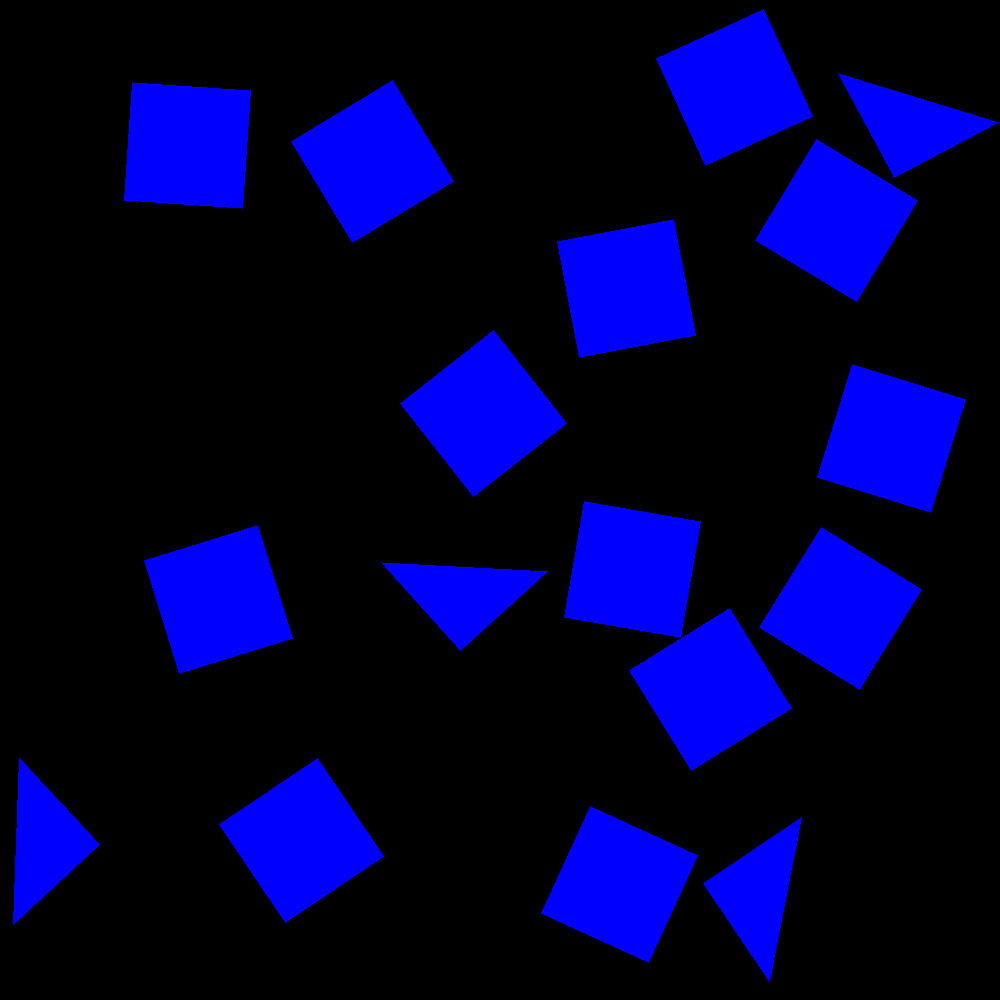
\includegraphics[width=2in, height=2in]{Counting/LaTeX/figures/putasideall/limitscaleresamplingoptionnetworkputaside/image1/touse/001.png} & 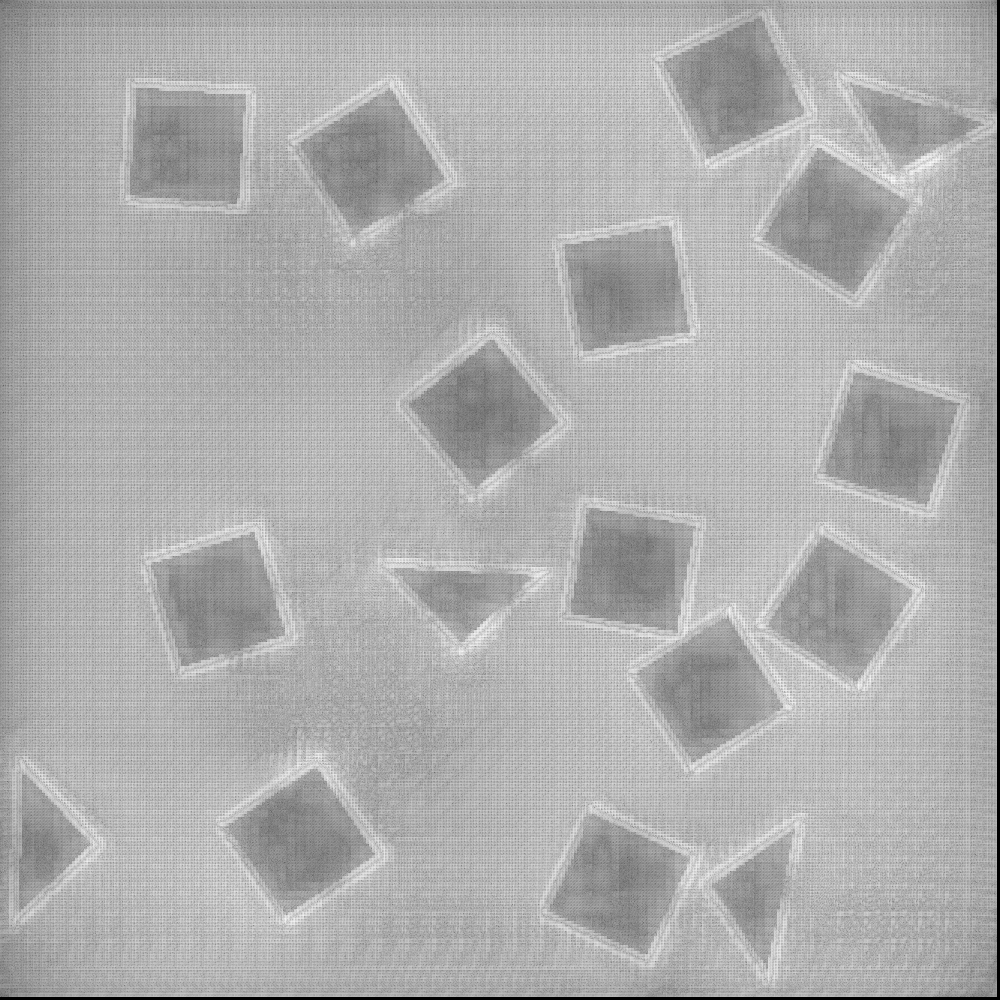
\includegraphics[width=2in, height=2in]{Counting/LaTeX/figures/putasideall/limitscaleresamplingoptionnetworkputaside/image1/touse/saliency.png} \\
            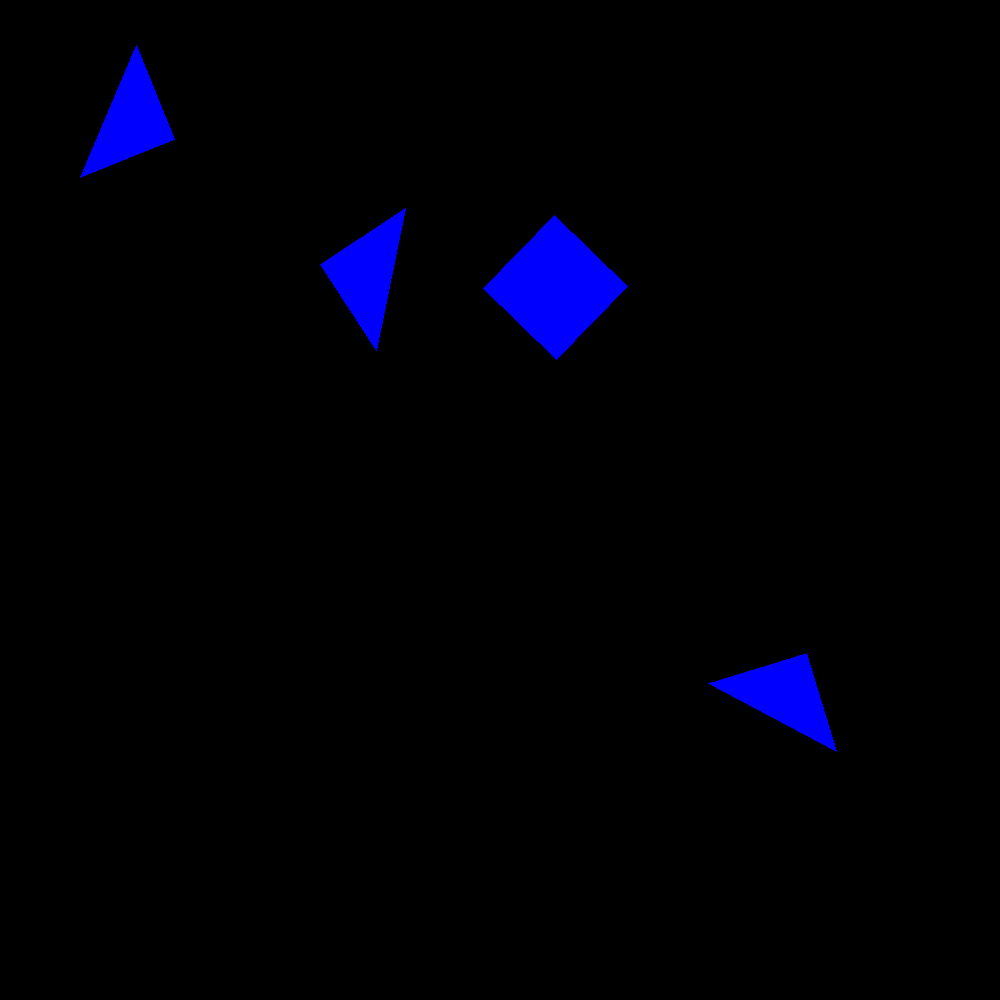
\includegraphics[width=2in, height=2in]{Counting/LaTeX/figures/putasideall/limitscaleresamplingoptionnetworkputaside/image2/touse/007.png} & 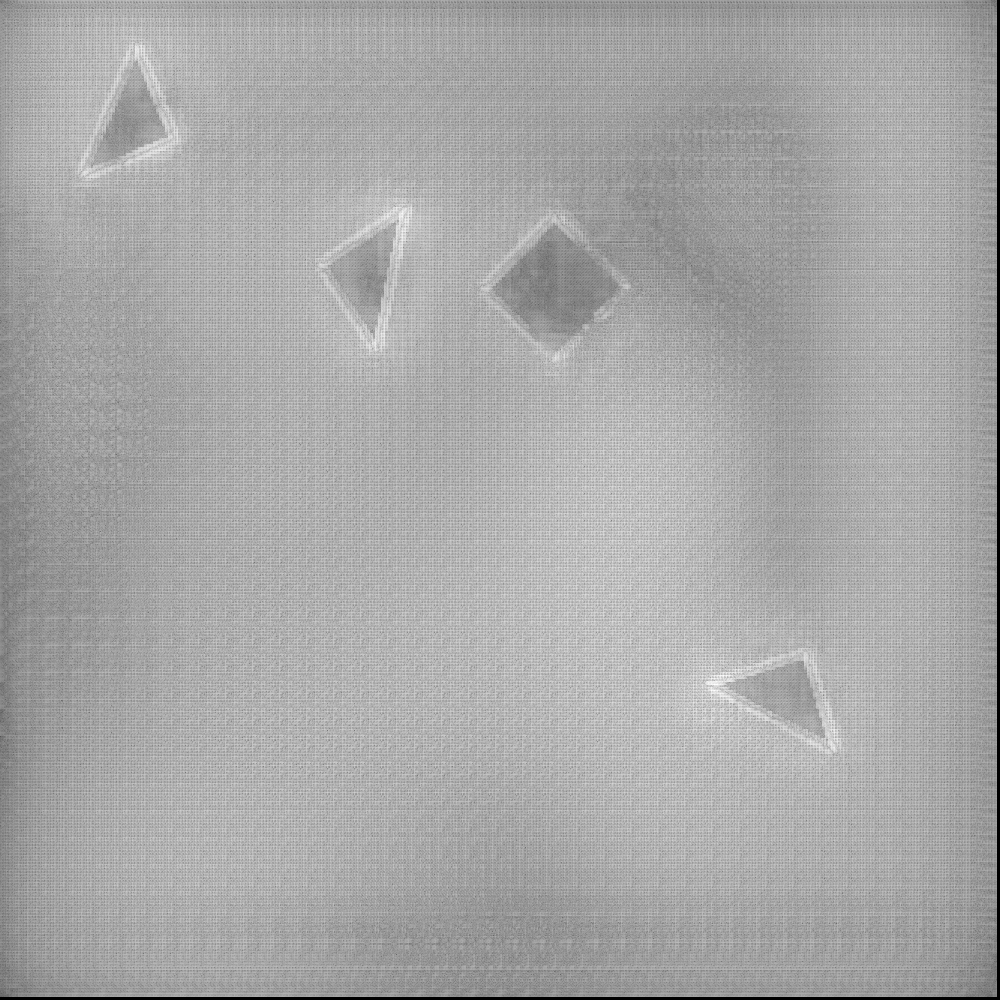
\includegraphics[width=2in, height=2in]{Counting/LaTeX/figures/putasideall/limitscaleresamplingoptionnetworkputaside/image2/touse/saliency.png}
        \end{tabular}
    \end{center}
    \caption{The first image is the image that the network sees, while the second image is the
             saliency for that image}
    \label{inputs}
\end{figure}

\begin{figure}[t]
    \begin{center}
        \begin{tabular}{c c c}
            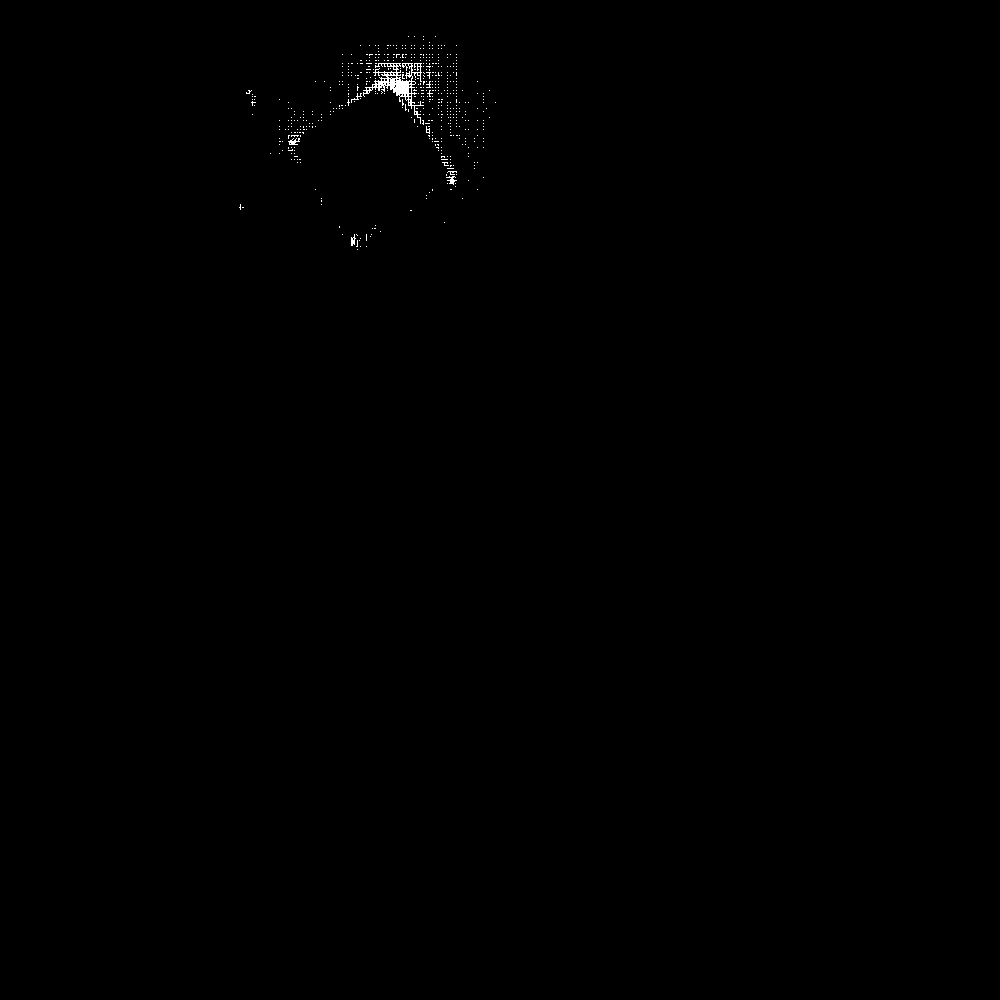
\includegraphics[width=1.5in, height=1.5in]{Counting/LaTeX/figures/putasideall/limitscaleresamplingoptionnetworkputaside/image1/touse/8.png}          & 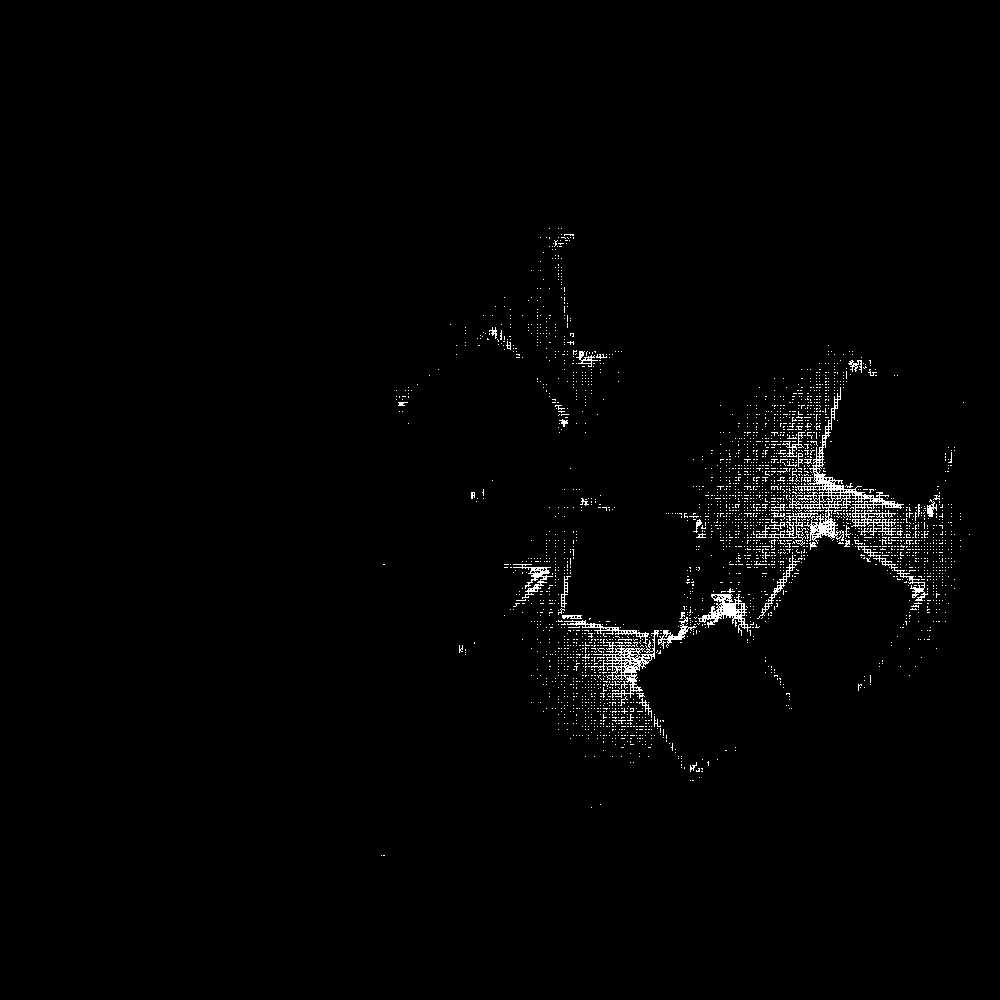
\includegraphics[width=1.5in, height=1.5in]{Counting/LaTeX/figures/putasideall/limitscaleresamplingoptionnetworkputaside/image1/touse/2.png}          & 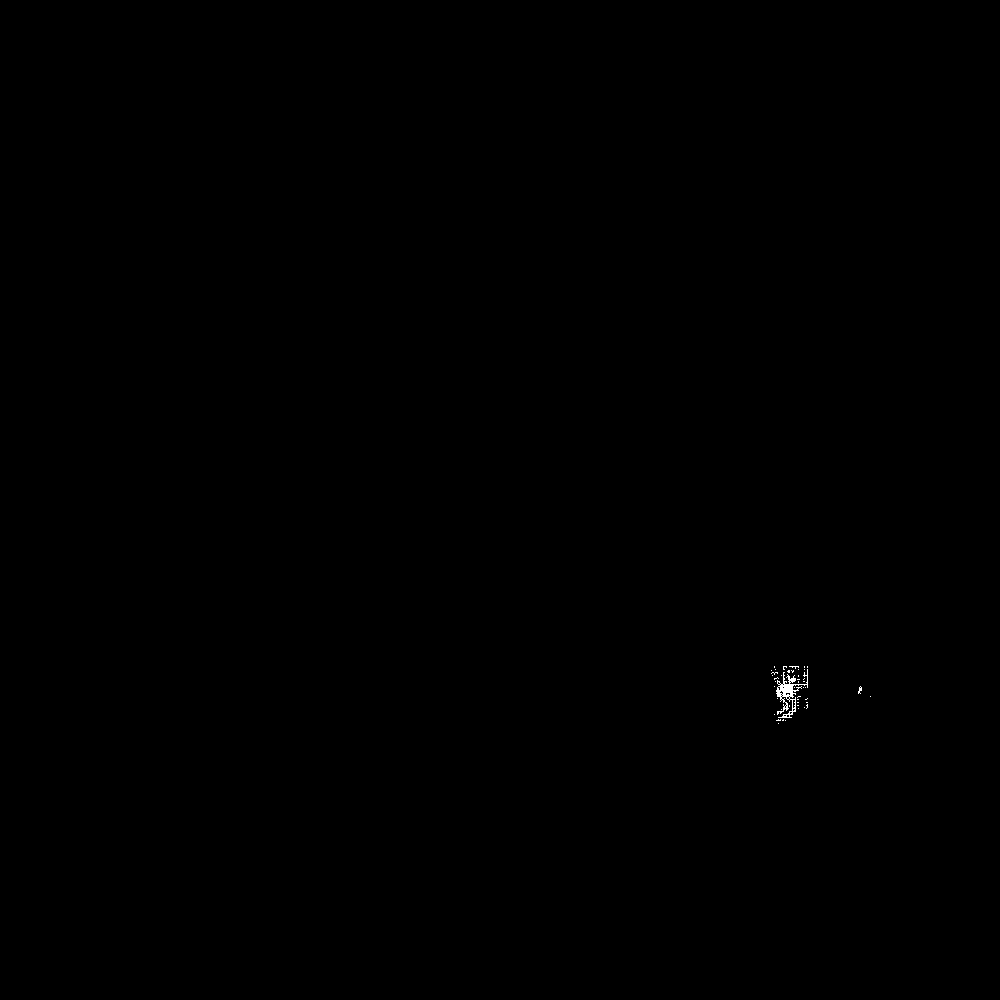
\includegraphics[width=1.5in, height=1.5in]{Counting/LaTeX/figures/putasideall/limitscaleresamplingoptionnetworkputaside/image1/touse/17.png}          \\
            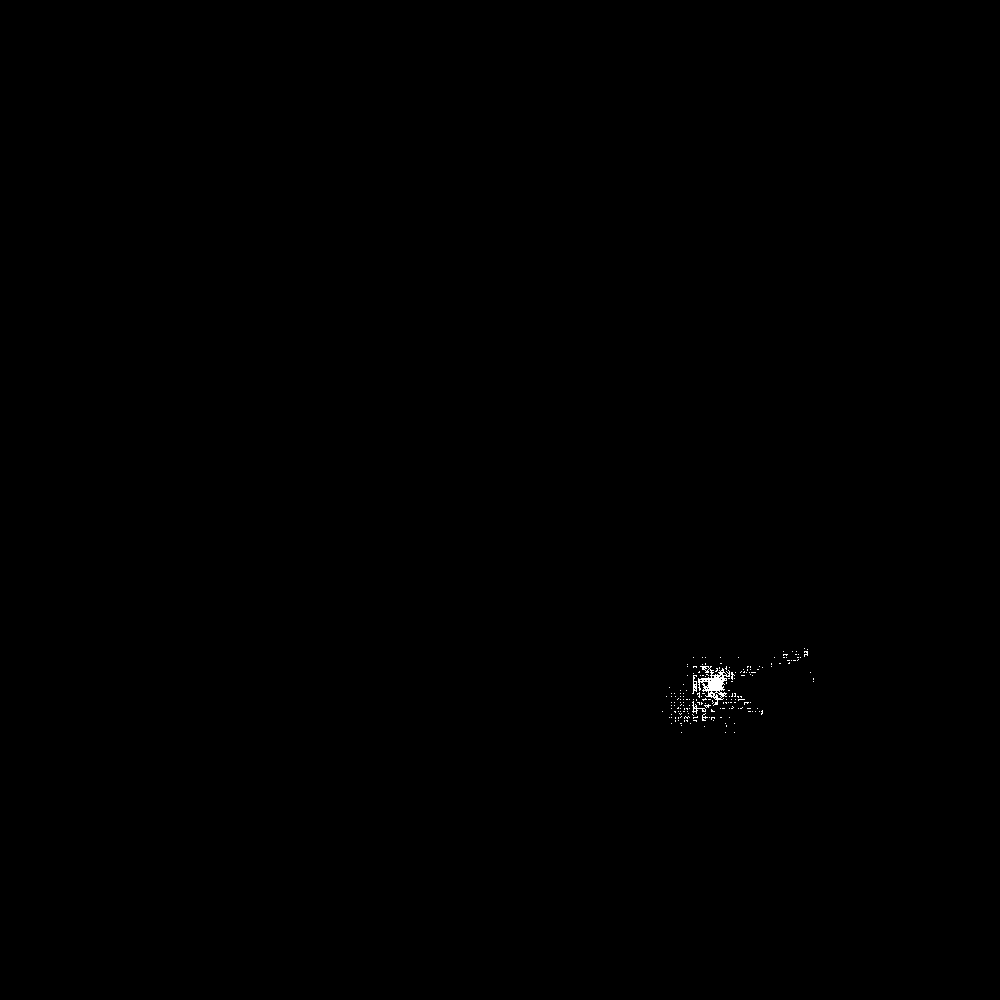
\includegraphics[width=1.5in, height=1.5in]{Counting/LaTeX/figures/putasideall/limitscaleresamplingoptionnetworkputaside/image2/touse/1.png}          & 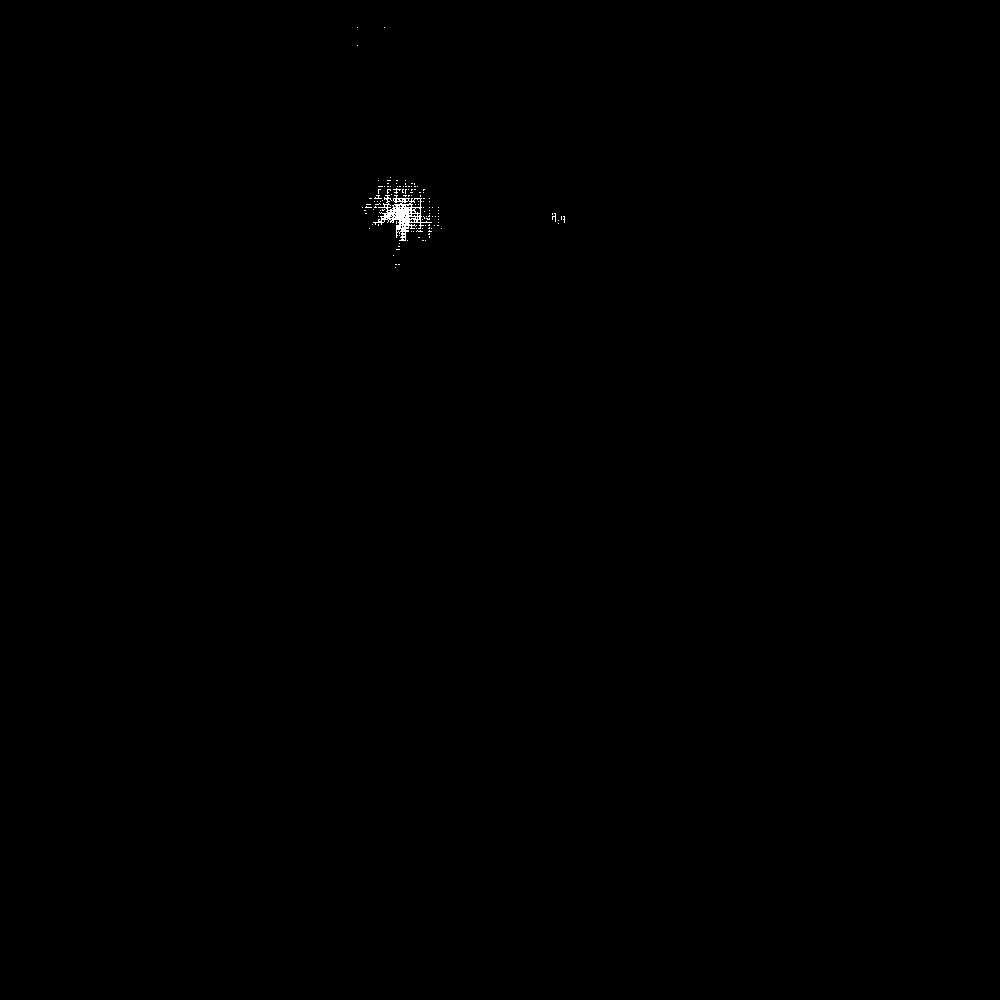
\includegraphics[width=1.5in, height=1.5in]{Counting/LaTeX/figures/putasideall/limitscaleresamplingoptionnetworkputaside/image2/touse/2.png}          & 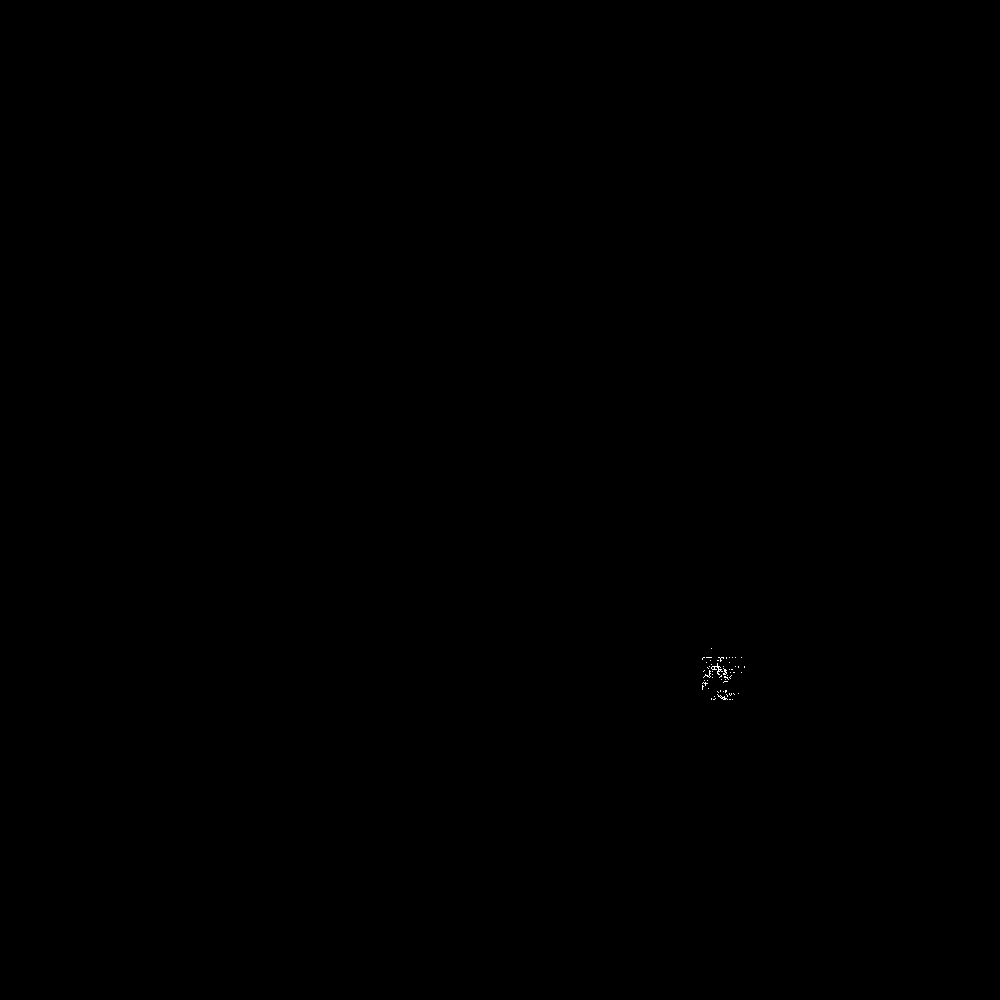
\includegraphics[width=1.5in, height=1.5in]{Counting/LaTeX/figures/putasideall/limitscaleresamplingoptionnetworkputaside/image2/touse/3.png}           \\
            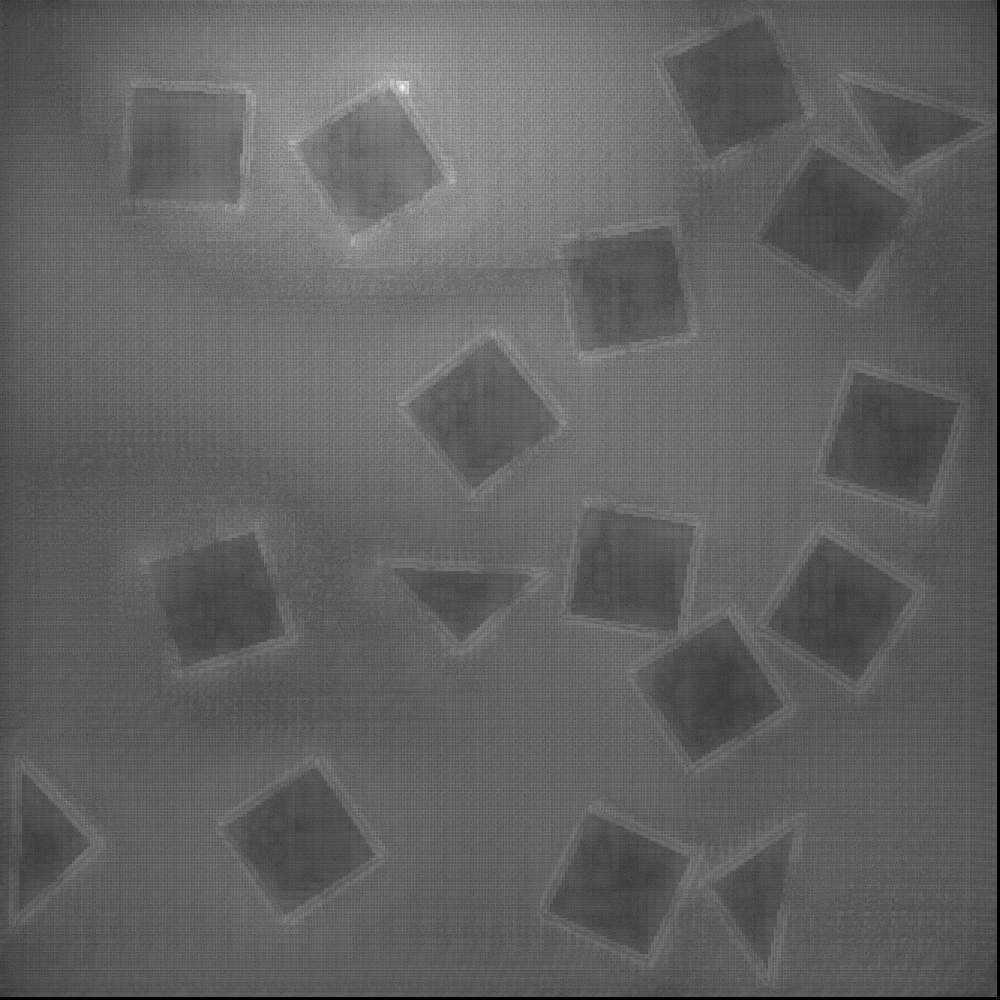
\includegraphics[width=1.5in, height=1.5in]{Counting/LaTeX/figures/putasideall/limitscaleresamplingoptionnetworkputaside/image1/touse/8-saliency.png} & 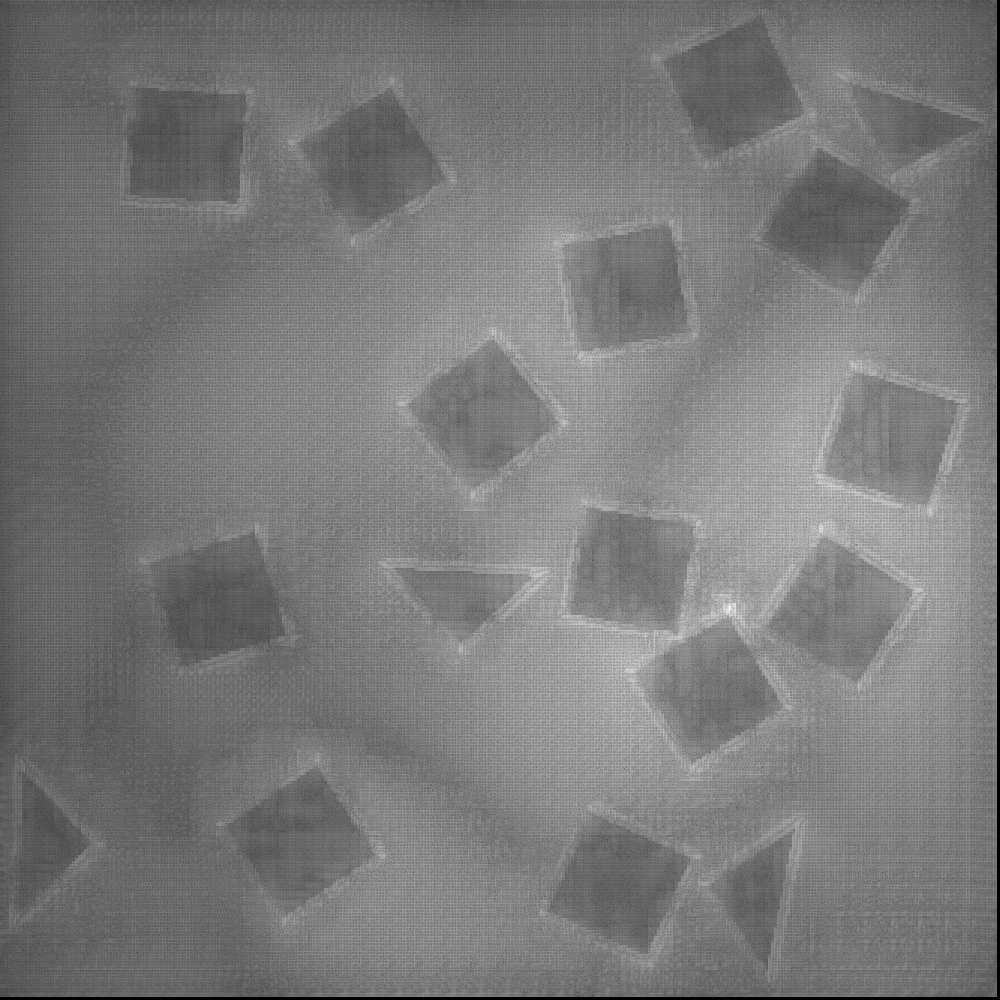
\includegraphics[width=1.5in, height=1.5in]{Counting/LaTeX/figures/putasideall/limitscaleresamplingoptionnetworkputaside/image1/touse/2-saliency.png} & 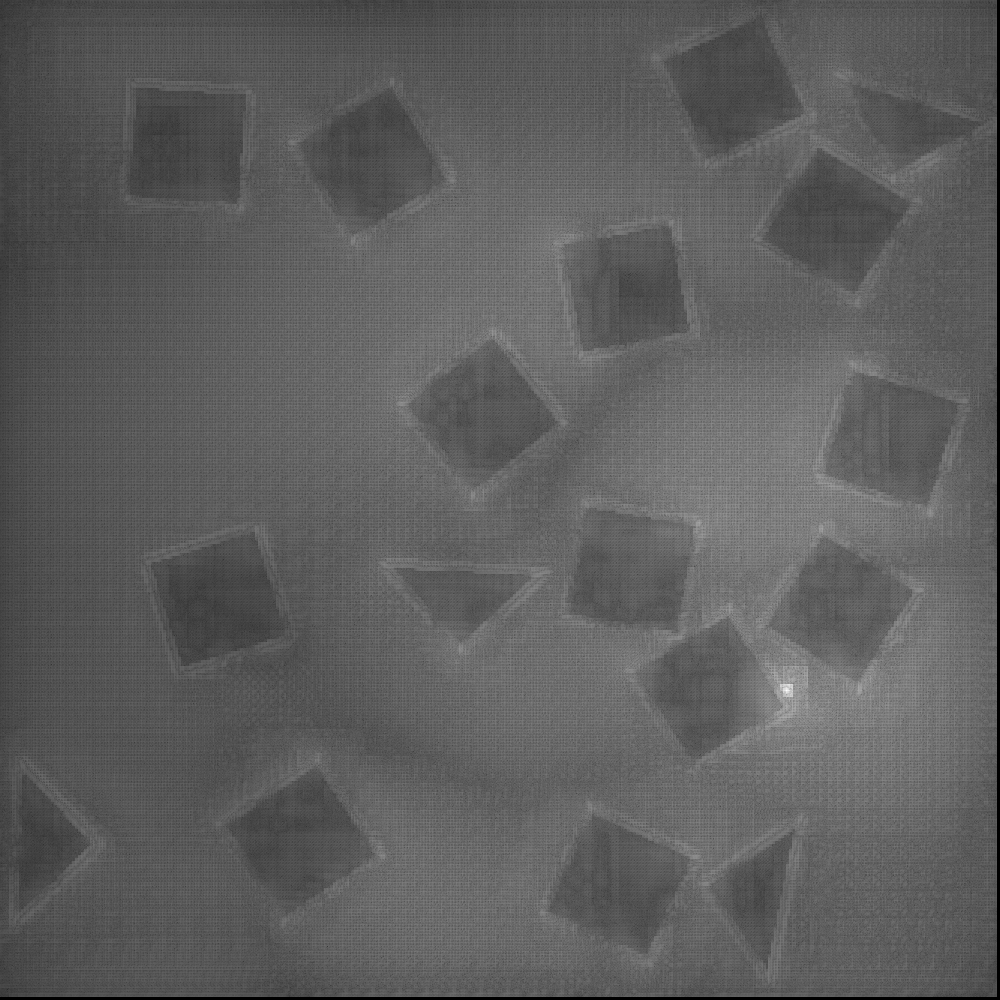
\includegraphics[width=1.5in, height=1.5in]{Counting/LaTeX/figures/putasideall/limitscaleresamplingoptionnetworkputaside/image1/touse/17-saliency.png} \\
            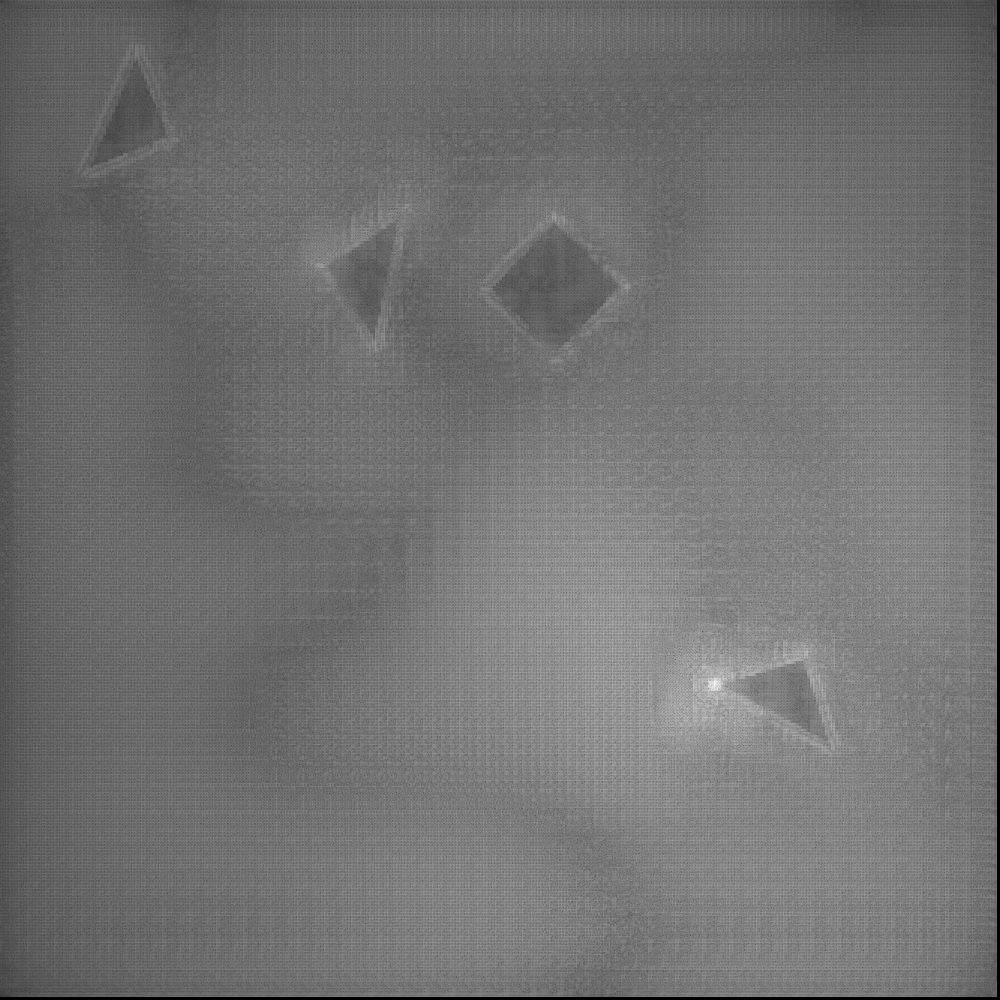
\includegraphics[width=1.5in, height=1.5in]{Counting/LaTeX/figures/putasideall/limitscaleresamplingoptionnetworkputaside/image2/touse/1-saliency.png} & 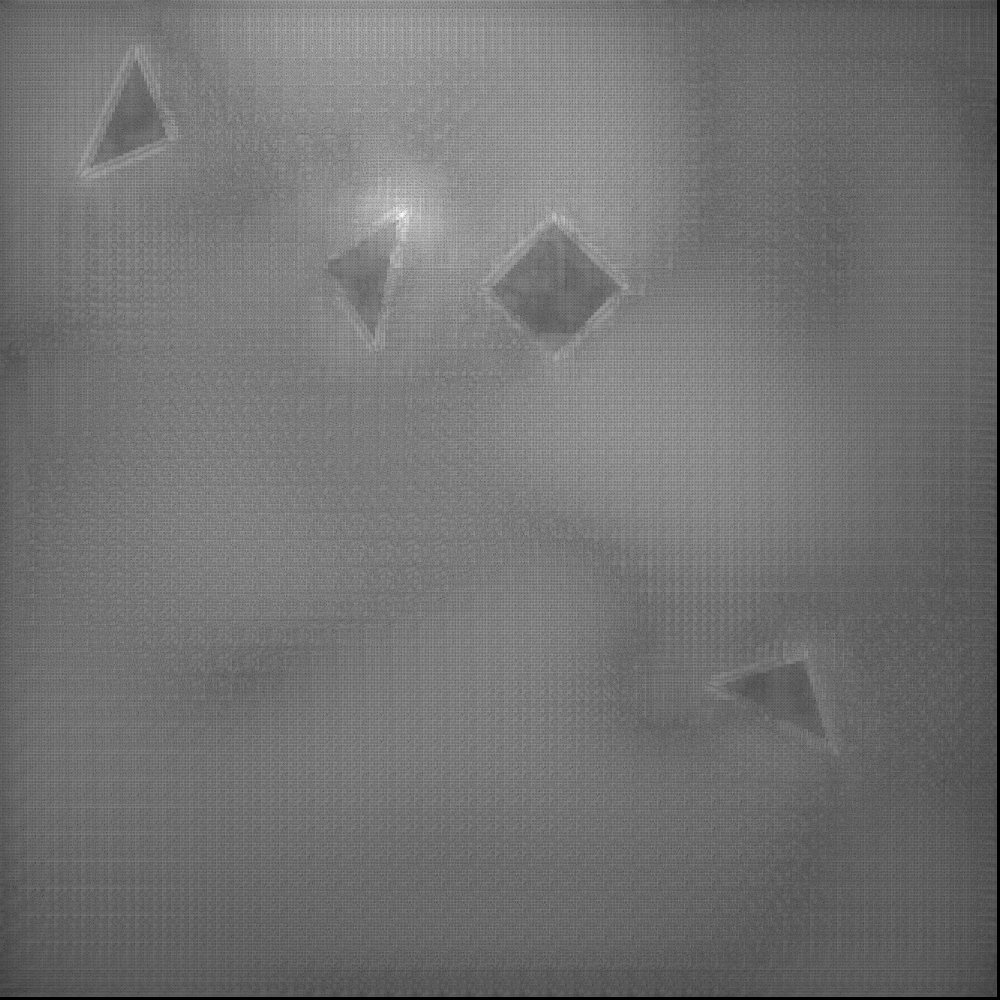
\includegraphics[width=1.5in, height=1.5in]{Counting/LaTeX/figures/putasideall/limitscaleresamplingoptionnetworkputaside/image2/touse/2-saliency.png} & 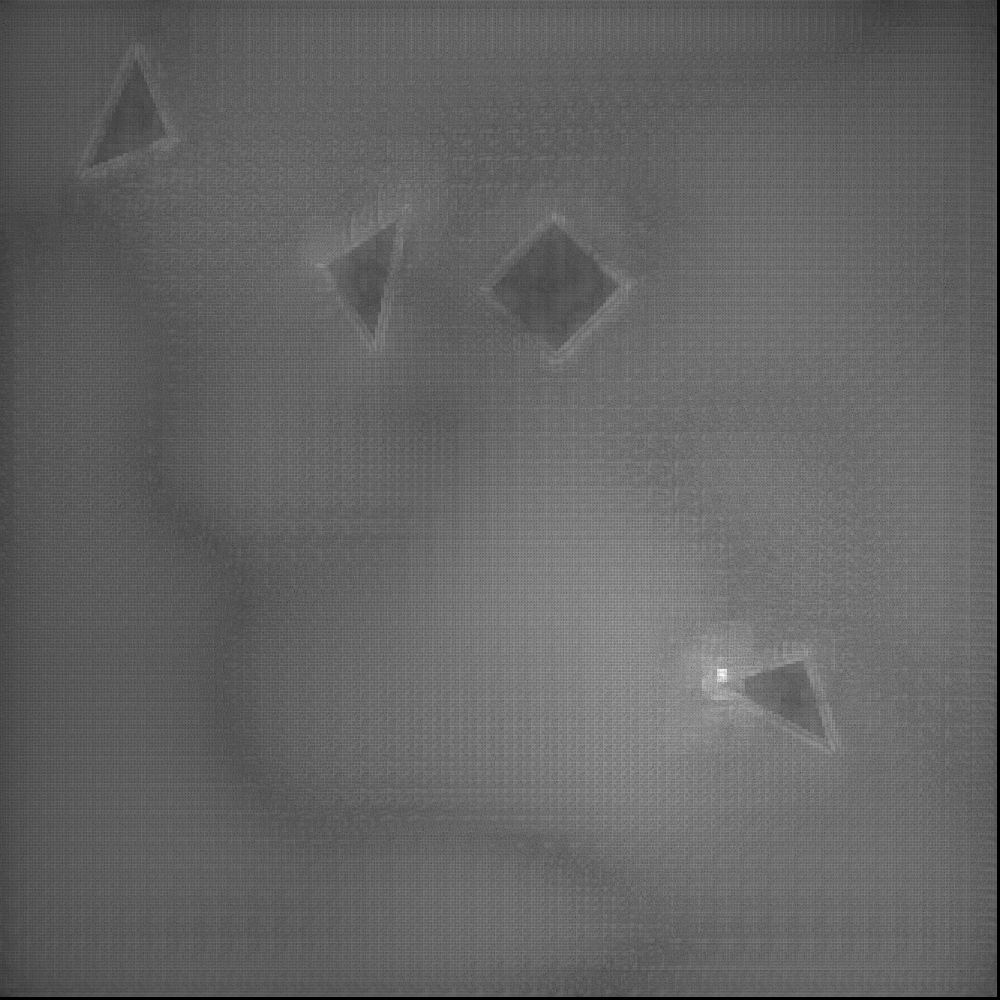
\includegraphics[width=1.5in, height=1.5in]{Counting/LaTeX/figures/putasideall/limitscaleresamplingoptionnetworkputaside/image2/touse/3-saliency.png}
        \end{tabular}
    \end{center}
    \caption{Each of the first two row represents a different image. The first images for these
             clearly shows the partial outline of a shape, while the second depicts the situation of
             a pixel being associated with multiple shapes. The third is the case where saliency
             selection derails and the area selected is not, or partially not, meaningful. Their
             full maps before thresholding are in the third and fourth rows.}
    \label{shapecorrelation}
\end{figure}



\subsection{Tweaks}



Initially, our ReLU-activated network was trained on images of shapes that did not vary in size.
Prediction was extremely accurate, so much so that it was suggested\footnote{by the author's
advisor, David Crandall} that the network may be effectively adding up the number of black pixels
(non-shape pixels) and dividing it by the number of pixels within a shape, or that corners were
being counted instead (a graph of the network output against the ground truth created with
\cite{Hunter:2007} when classifying both shapes and squares confirmed this). To ameliorate this
issue, the network was trained on shapes of different sizes and was restructured to be
bigger\footnote{David Crandall implied that capacity might be a potential issue}. The ability of the
network to predict correctly was significantly reduced but was not bad, initially indicating that
the network had learned some kind of representation of the shapes. Further, it gave us saliency maps
that appeared to be what we were looking for, which was that the network learned the representation
of the shapes itself (see figure \ref{initialsaliency}). However, due to the problem of the second
derivative mentioned above, the second derivative did not give us anything meaningful. As a result,
SoftPlus~\cite{NIPS2000_44968aec} was tried, but this resulted in numerical issues that sill might
have squeaked some interesting detection pixels (see figure \ref{norenormalizationsoftplus}).

\begin{figure}
    \begin{center}
        \begin{tabular}{c c}
            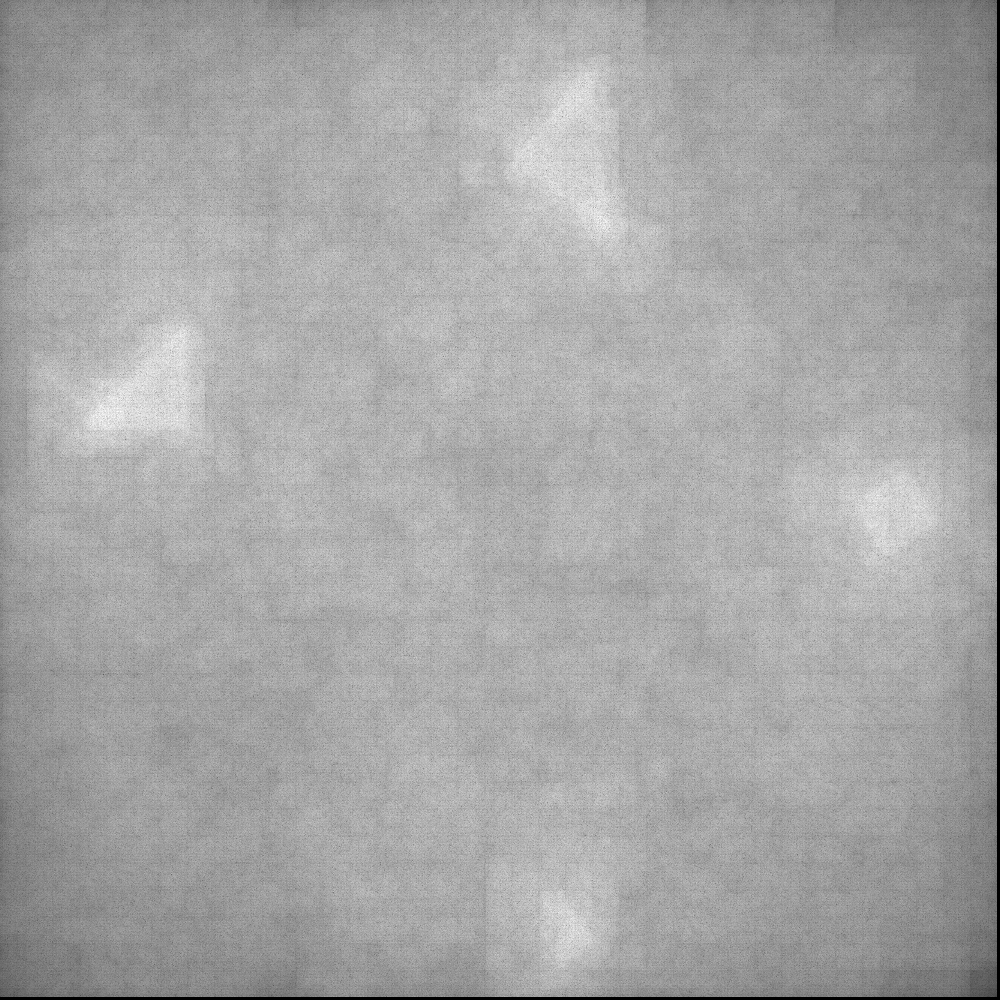
\includegraphics[width = 3in, height = 3in]{Counting/LaTeX/figures/putasideall/nolimitscaleresamplingoptiondifferentactivation2networkputaside/image1/saliency.png} & 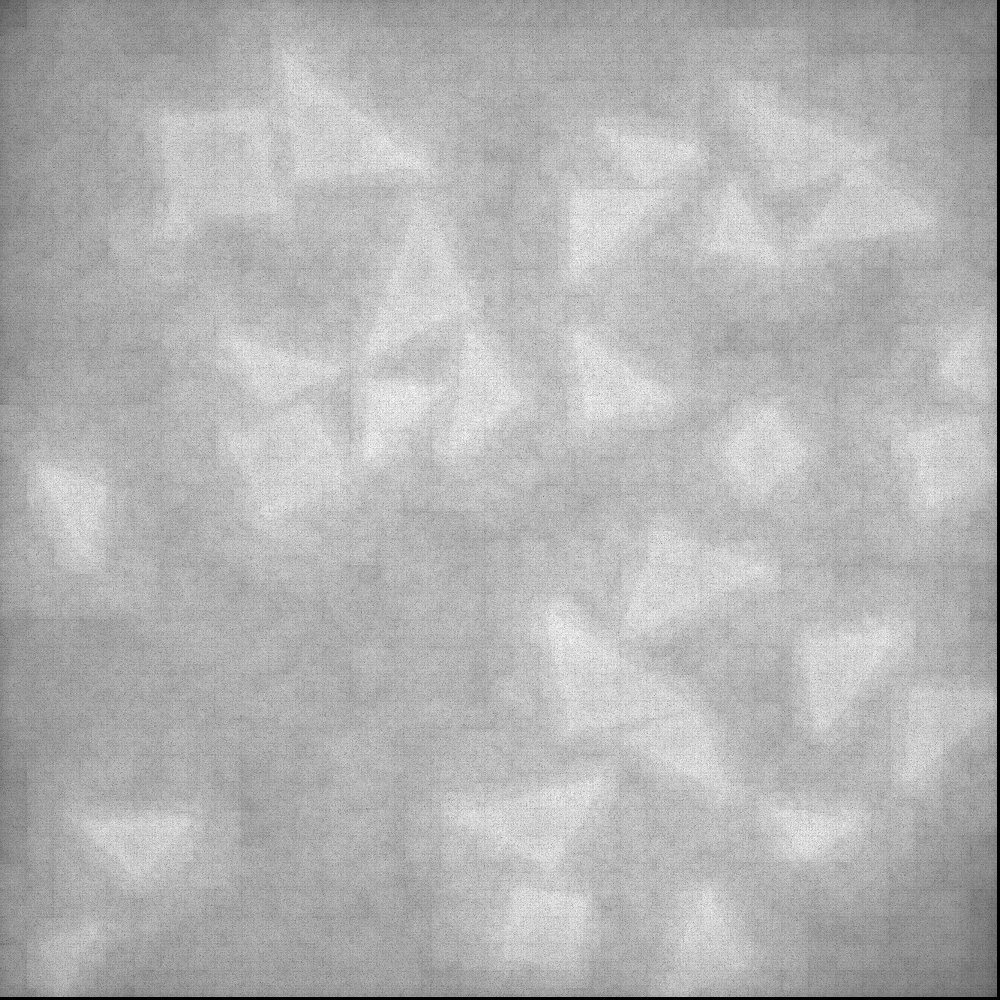
\includegraphics[width = 3in, height = 3in]{Counting/LaTeX/figures/putasideall/nolimitscaleresamplingoptiondifferentactivation2networkputaside/image2/saliency.png}
        \end{tabular}
    \end{center}
    \caption{ReLU-based saliency.}
    \label{initialsaliency}
\end{figure}

\begin{figure}
    \begin{center}
        \begin{tabular}{c c}
            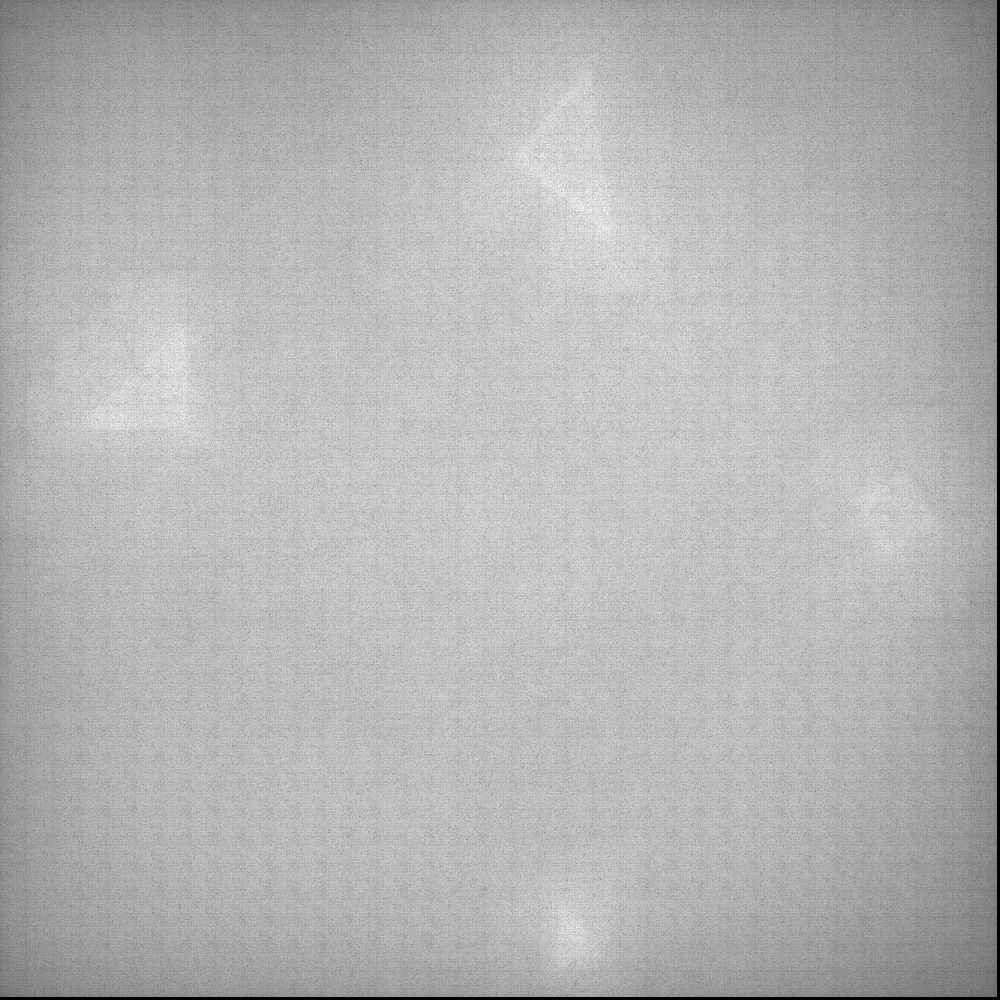
\includegraphics[width = 3in, height = 3in]{Counting/LaTeX/figures/putasideall/nolimitscaleresamplingoptiondifferentactivation3networkputaside/image1/saliency.png} & 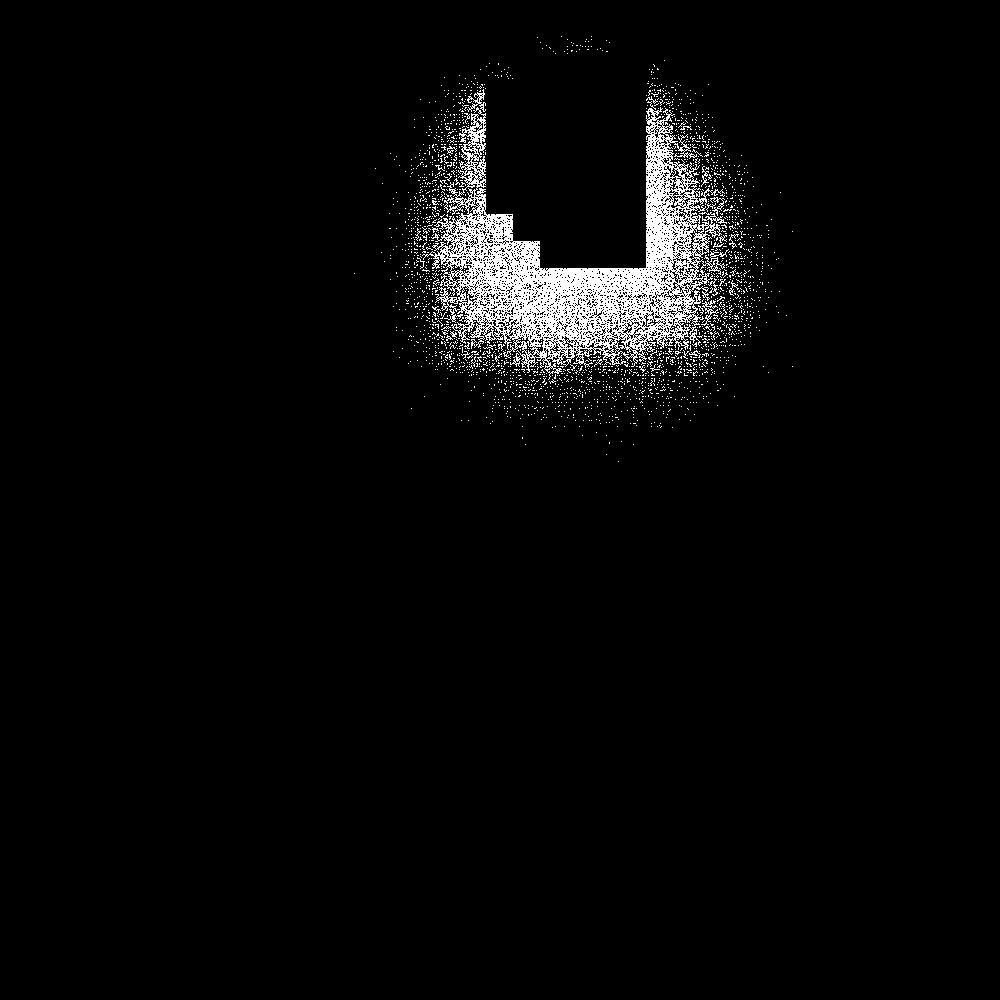
\includegraphics[width = 3in, height = 3in]{Counting/LaTeX/figures/putasideall/nolimitscaleresamplingoptiondifferentactivation3networkputaside/image1/1.png}
        \end{tabular}
    \end{center}
    \caption{Our first attempt at using SoftPlus~\cite{NIPS2000_44968aec}}
    \label{norenormalizationsoftplus}
\end{figure}

We moved to a sigmoid activation function (although we are not entirely sure why), with the network
trained with Batch Renormalization~\cite{ioffe2017batch} (to get the sigmoid network to actually
converge), but that only put the saliency in the blank space of the image. This is shown in figure
\ref{badsaliency}. This remained a frustrating issue until we found \cite{guan2021understanding},
which states ``[a]lthough sizes are random in a range, the average size...stabl[izes] [as] the
number of objects increases''~\cite{guan2021understanding}[page 3]. As a result, for two images that
have the same counts, the number of relevant pixels will remain the same, which makes the network's
job as easy as counting pixels. Therefore, we implemented the solution that they proposed, which was
to use randomly-sized shapes, with all the shapes in the image taking on that random size. Size
resampling happens after each image is generated. In \cite{guan2021understanding}, they allocated a
static number of pixels to the image, and thus the size of the shape depended on how many shapes
were to be put in that image. However, we made a slight tweak: we decoupled the number of shapes
from limit on the number of pixels, and just made sure to pick a range of scales that allowed all
the shapes to fit in a worst-case scenario (this was likely the problem they were trying to avoid by
imposing the aforementioned limit). We decided to go this way because it seemed less likely that the
neural network would find another non-optimal way to regress. The result from this method is
discussed in the previous section.

\begin{figure}
    \begin{center}
        \begin{tabular}{c c}
            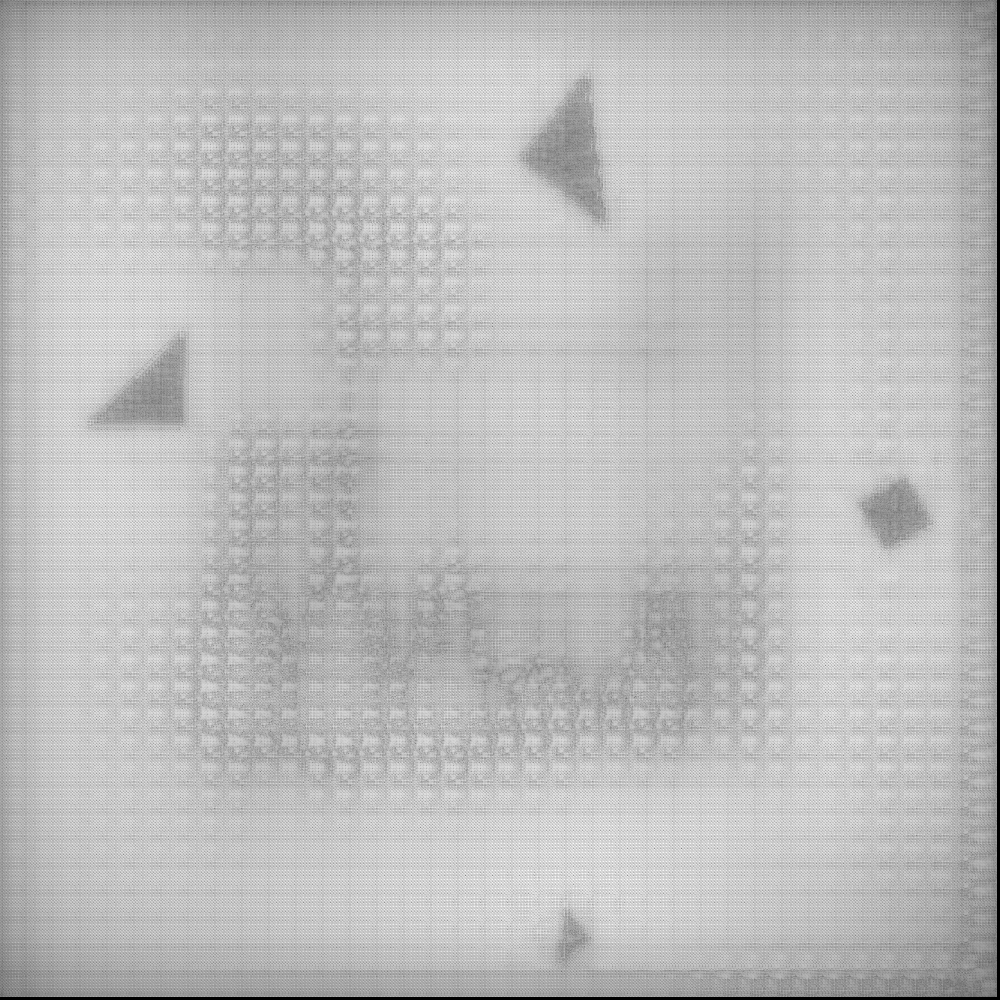
\includegraphics[width = 2.3in, height = 2.3in]{Counting/LaTeX/figures/putasideall/nolimitscaleresamplingoptiondifferentactivationnetworkputaside/image1/saliency.png}   & 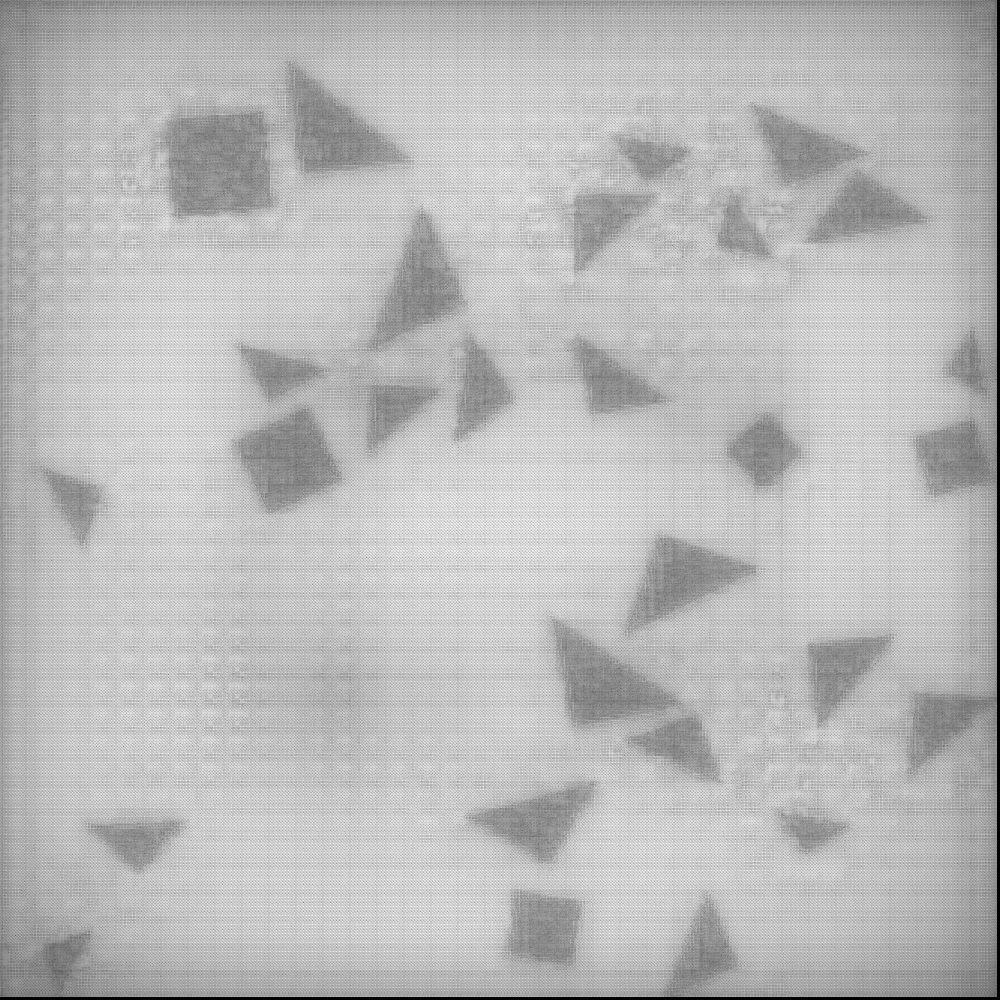
\includegraphics[width = 2.3in, height = 2.3in]{Counting/LaTeX/figures/putasideall/nolimitscaleresamplingoptiondifferentactivationnetworkputaside/image2/saliency.png} \\
            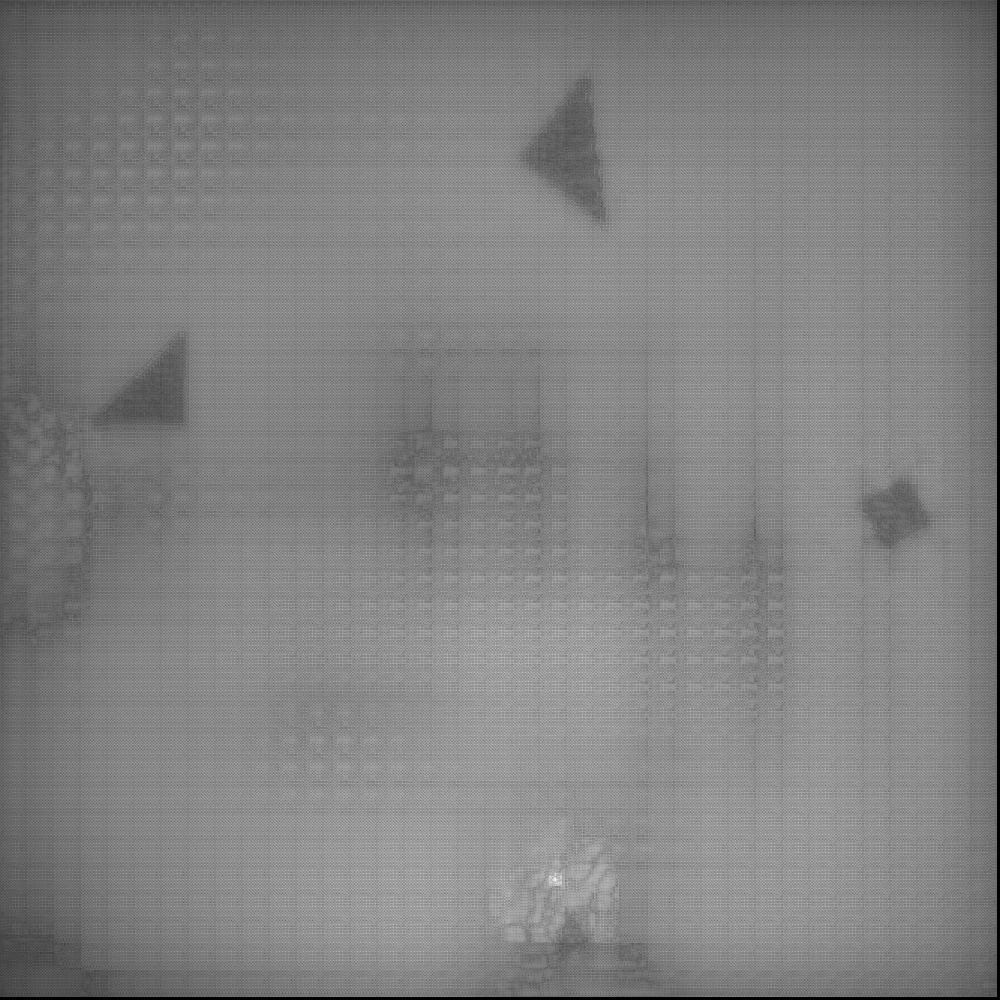
\includegraphics[width = 2.3in, height = 2.3in]{Counting/LaTeX/figures/putasideall/nolimitscaleresamplingoptiondifferentactivationnetworkputaside/image1/1-saliency.png}   & 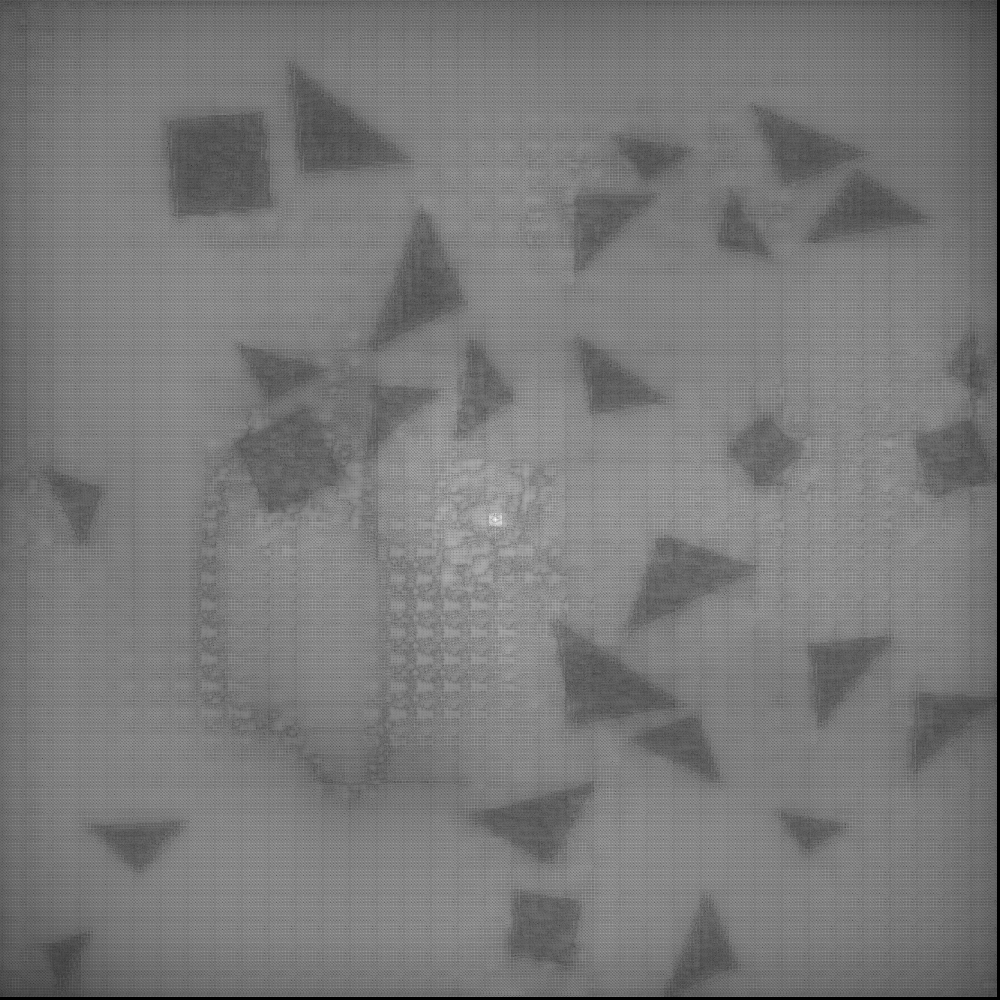
\includegraphics[width = 2.3in, height = 2.3in]{Counting/LaTeX/figures/putasideall/nolimitscaleresamplingoptiondifferentactivationnetworkputaside/image2/1-saliency.png} \\
            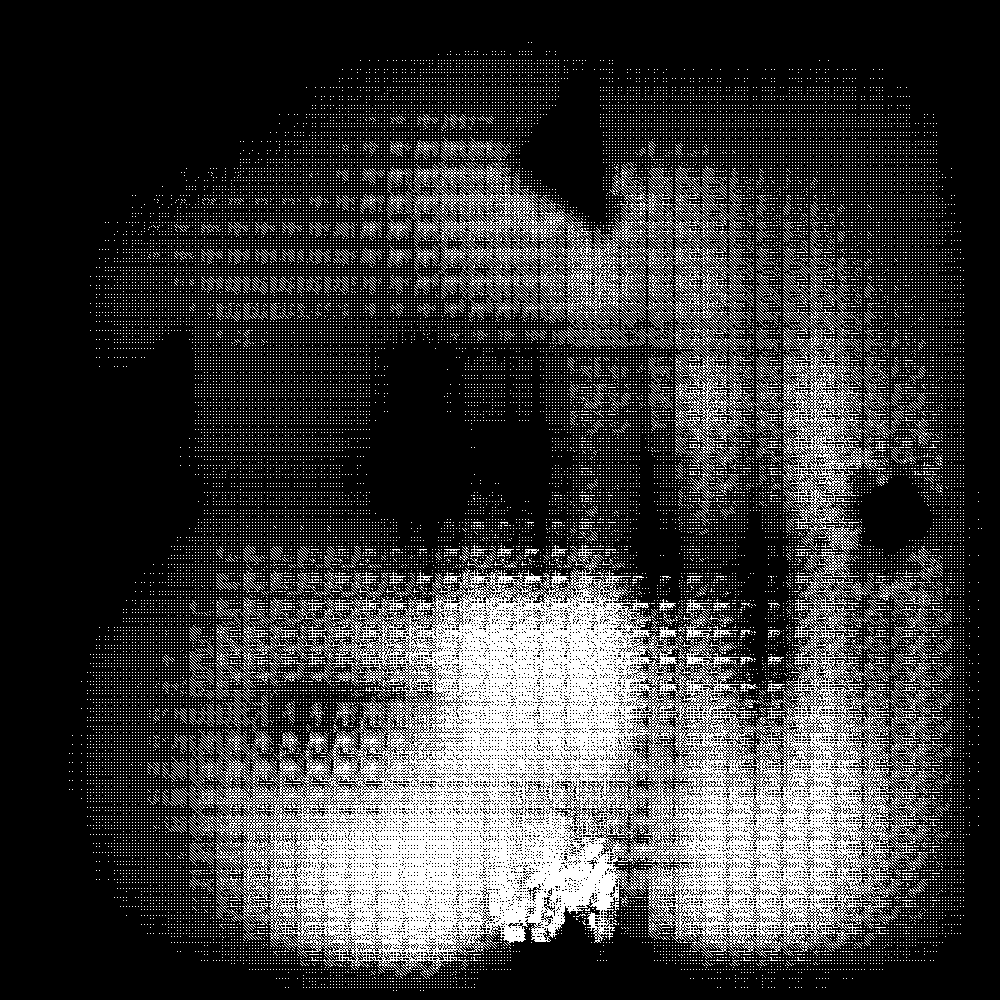
\includegraphics[width = 2.3in, height = 2.3in]{Counting/LaTeX/figures/putasideall/nolimitscaleresamplingoptiondifferentactivationnetworkputaside/image1/1.png} & 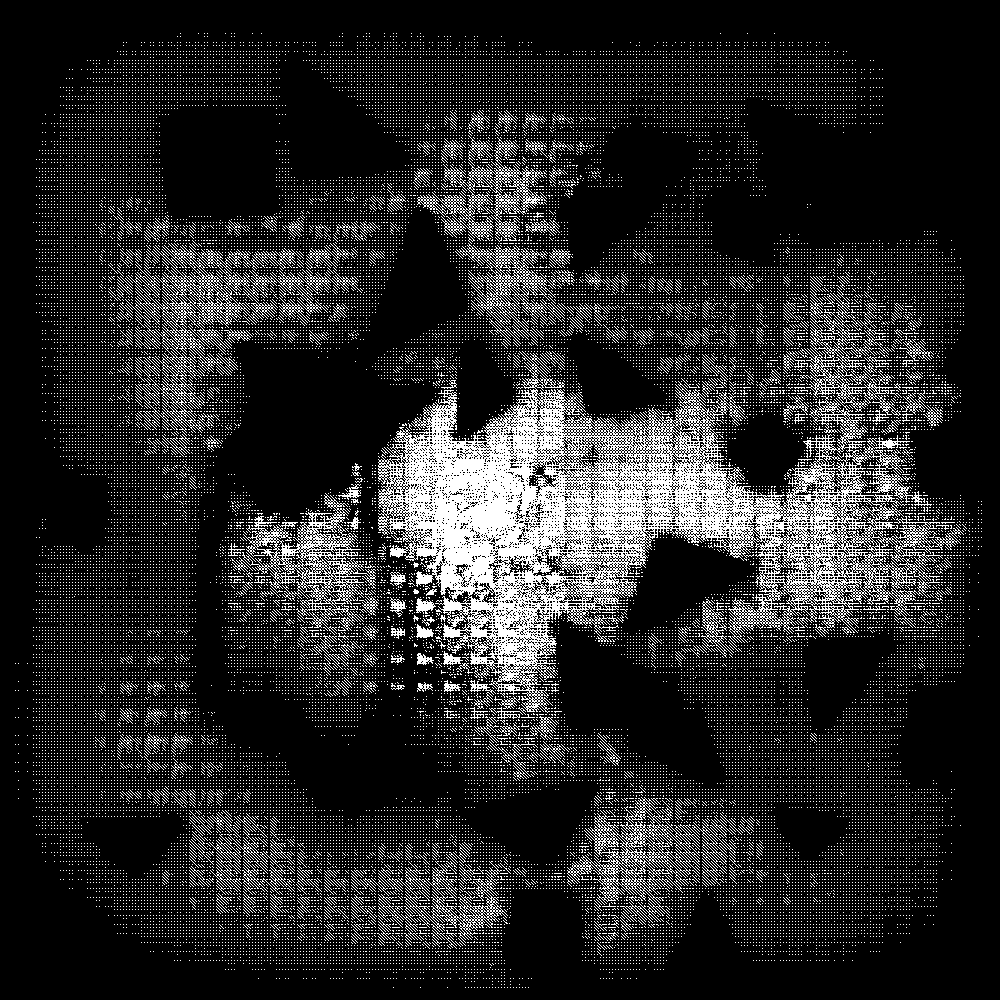
\includegraphics[width = 2.3in, height = 2.3in]{Counting/LaTeX/figures/putasideall/nolimitscaleresamplingoptiondifferentactivationnetworkputaside/image2/1.png}
        \end{tabular}
    \end{center}
    \caption{The first row shows saliency maps for two images, the second row shows the connection
             strength between the most salient pixel and others, and the third row are the pixels
             that ``qualify'' as being part of a shape}
    \label{badsaliency}
\end{figure}





Further tweaks need to address the problem discussed in section \ref{algorithm}. Regarding the most
salient pixels being between shapes, it may be necessary to modify the loss function from which to
backpropagate. Candidates would need to encode encouraging strong gradients that \textit{only}
relate to decreasing the count by one. Another option is to threshold the first derivative saliency
from above. As a result, errant pixels in the gap between shapes with large saliency would not be
considered. Further, as stated previously, automatic determination of both thresholds would be
substantially better than manual settings. This would become even more crucial when tackling
real-world issues. An alternative solution may be to use K-means to group low, medium and high
saliency pixels. The idea is that we would only stick with the medium-saliency pixels as the high
saliency group would have many pixels that may change the count too much; rejecting those with low
saliency values was justified previously. One may need to consider the distance metric to be used;
for example, high saliency pixels may be distributed in an exponential fashion, so normal Euclidean
distance would leave many undesired saliencies in the acceptable group.

Further, it is important to point out that real-world circumstances may actually provide
\textit{better, more reliable} saliency values. Counting shapes may have a significant flaw, which
is that ordinary, monocolor shapes really don't have many features outside of their edges and
corners\footnote{David Crandall reminded me about corners possibly being important.}. If there are
features that are internal to the object, it may result in cleaner saliency values that are focused
on the object itself. However, it is also possible that the network learns to identify one component
that many objects in the image share, and, as a result, its children pixels do not span the object
entirely, making bounding box prediction problematic.

Our code and models can be found in the "Counting" folder at \cite{mycode}.
